\section{前言}

中国水果产业品类多、总量大，水果产业已经成为了中国继粮食、蔬菜之后的第三农业种植产业，果园总面积和水果总产量年稳居世界首位。我国果品的生产总量、栽培面积及资源种类均居于世界首位，国家统计局数据显示，2022年，中国水果产量为31296.24万吨，同比增长4.42\%。我国虽然是世界水果生产大国之一，但并不是世界水，果生产强国\cite{__2022}，我国水果产业没有充分发挥我国所有的自然资源优势。其中，我国水果出口贸易发展中存在的国际影响力弱，水果竞争力弱等问题，最根本的原因是我国果品品质差、劣质品种多。

水果产业的优质发展不仅需要充足的营养，还需要有良好的果园管理技术和方法。果园管理中土壤的养分管理尤其重要，土壤养分条件决定了果品质量以及果园可持续发展\cite{hoagland_orchard_2008}。土壤有机质对果树优质生长发挥了重大的作用\cite{sun_fruit_2022}\cite{_123_2020}，它富含养分，保证土壤养分供应，支撑水分净化、保持和供应\cite{kay_sensitivity_1997}。施用有机肥可以提高微生物群落的生态稳定性、促进果树作物的光合作用，因此施用有机肥对提升果实品质和保护生态环境有着重大意义\cite{__2024}\cite{__2021}。

果园施肥机械化可以减少生产管理成本，提高施肥作业效率和施肥质量，促进果园肥料高速利用，实现果园增产\cite{__2020}。长久以来我国有机肥施肥方式以人工方式为主，成本较高、劳动强度大\cite{__2016}。如图\ref{pic:课题组先前研制的有机肥施肥机}所示，课题组先前研究的施肥机施肥过程中易出现肥料与箱底粘附，导致排肥装置工作阻力增大，最终造成有机肥堵塞影响施肥机正常施肥等问题。这是由于有机肥流动性差和含有一定水分的特性导致的，有机肥如图\ref{pic:有机肥}所示。由于农业机械与作物、肥料与土壤等接触作业产生的阻力消耗了大量的动力和能源，因此减阻始终是农业机械设计领域的首要目标\cite{__2017}。

\begin{figure}[H]
	\centering
	\begin{minipage}[b]{0.45\textwidth}
		\centering
		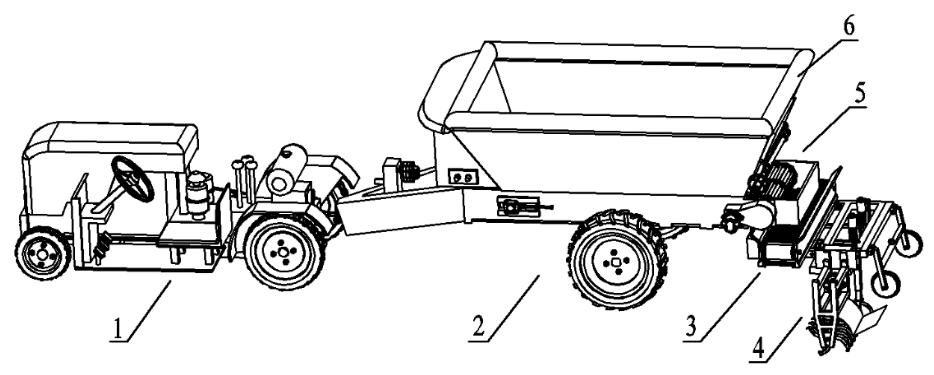
\includegraphics[width=0.45\textwidth]{../../assets/课题组先前研制的有机肥施肥机.png}

		{\small 1-拖拉机；2-施肥车；3-抛肥装置；

		4-肥土混合部件；5-排肥装置；6-肥箱；}

		\caption{课题组先前研制的有机肥施肥机}
		\label{pic:课题组先前研制的有机肥施肥机}
	\end{minipage}
	\begin{minipage}[b]{0.45\textwidth}
		\centering
		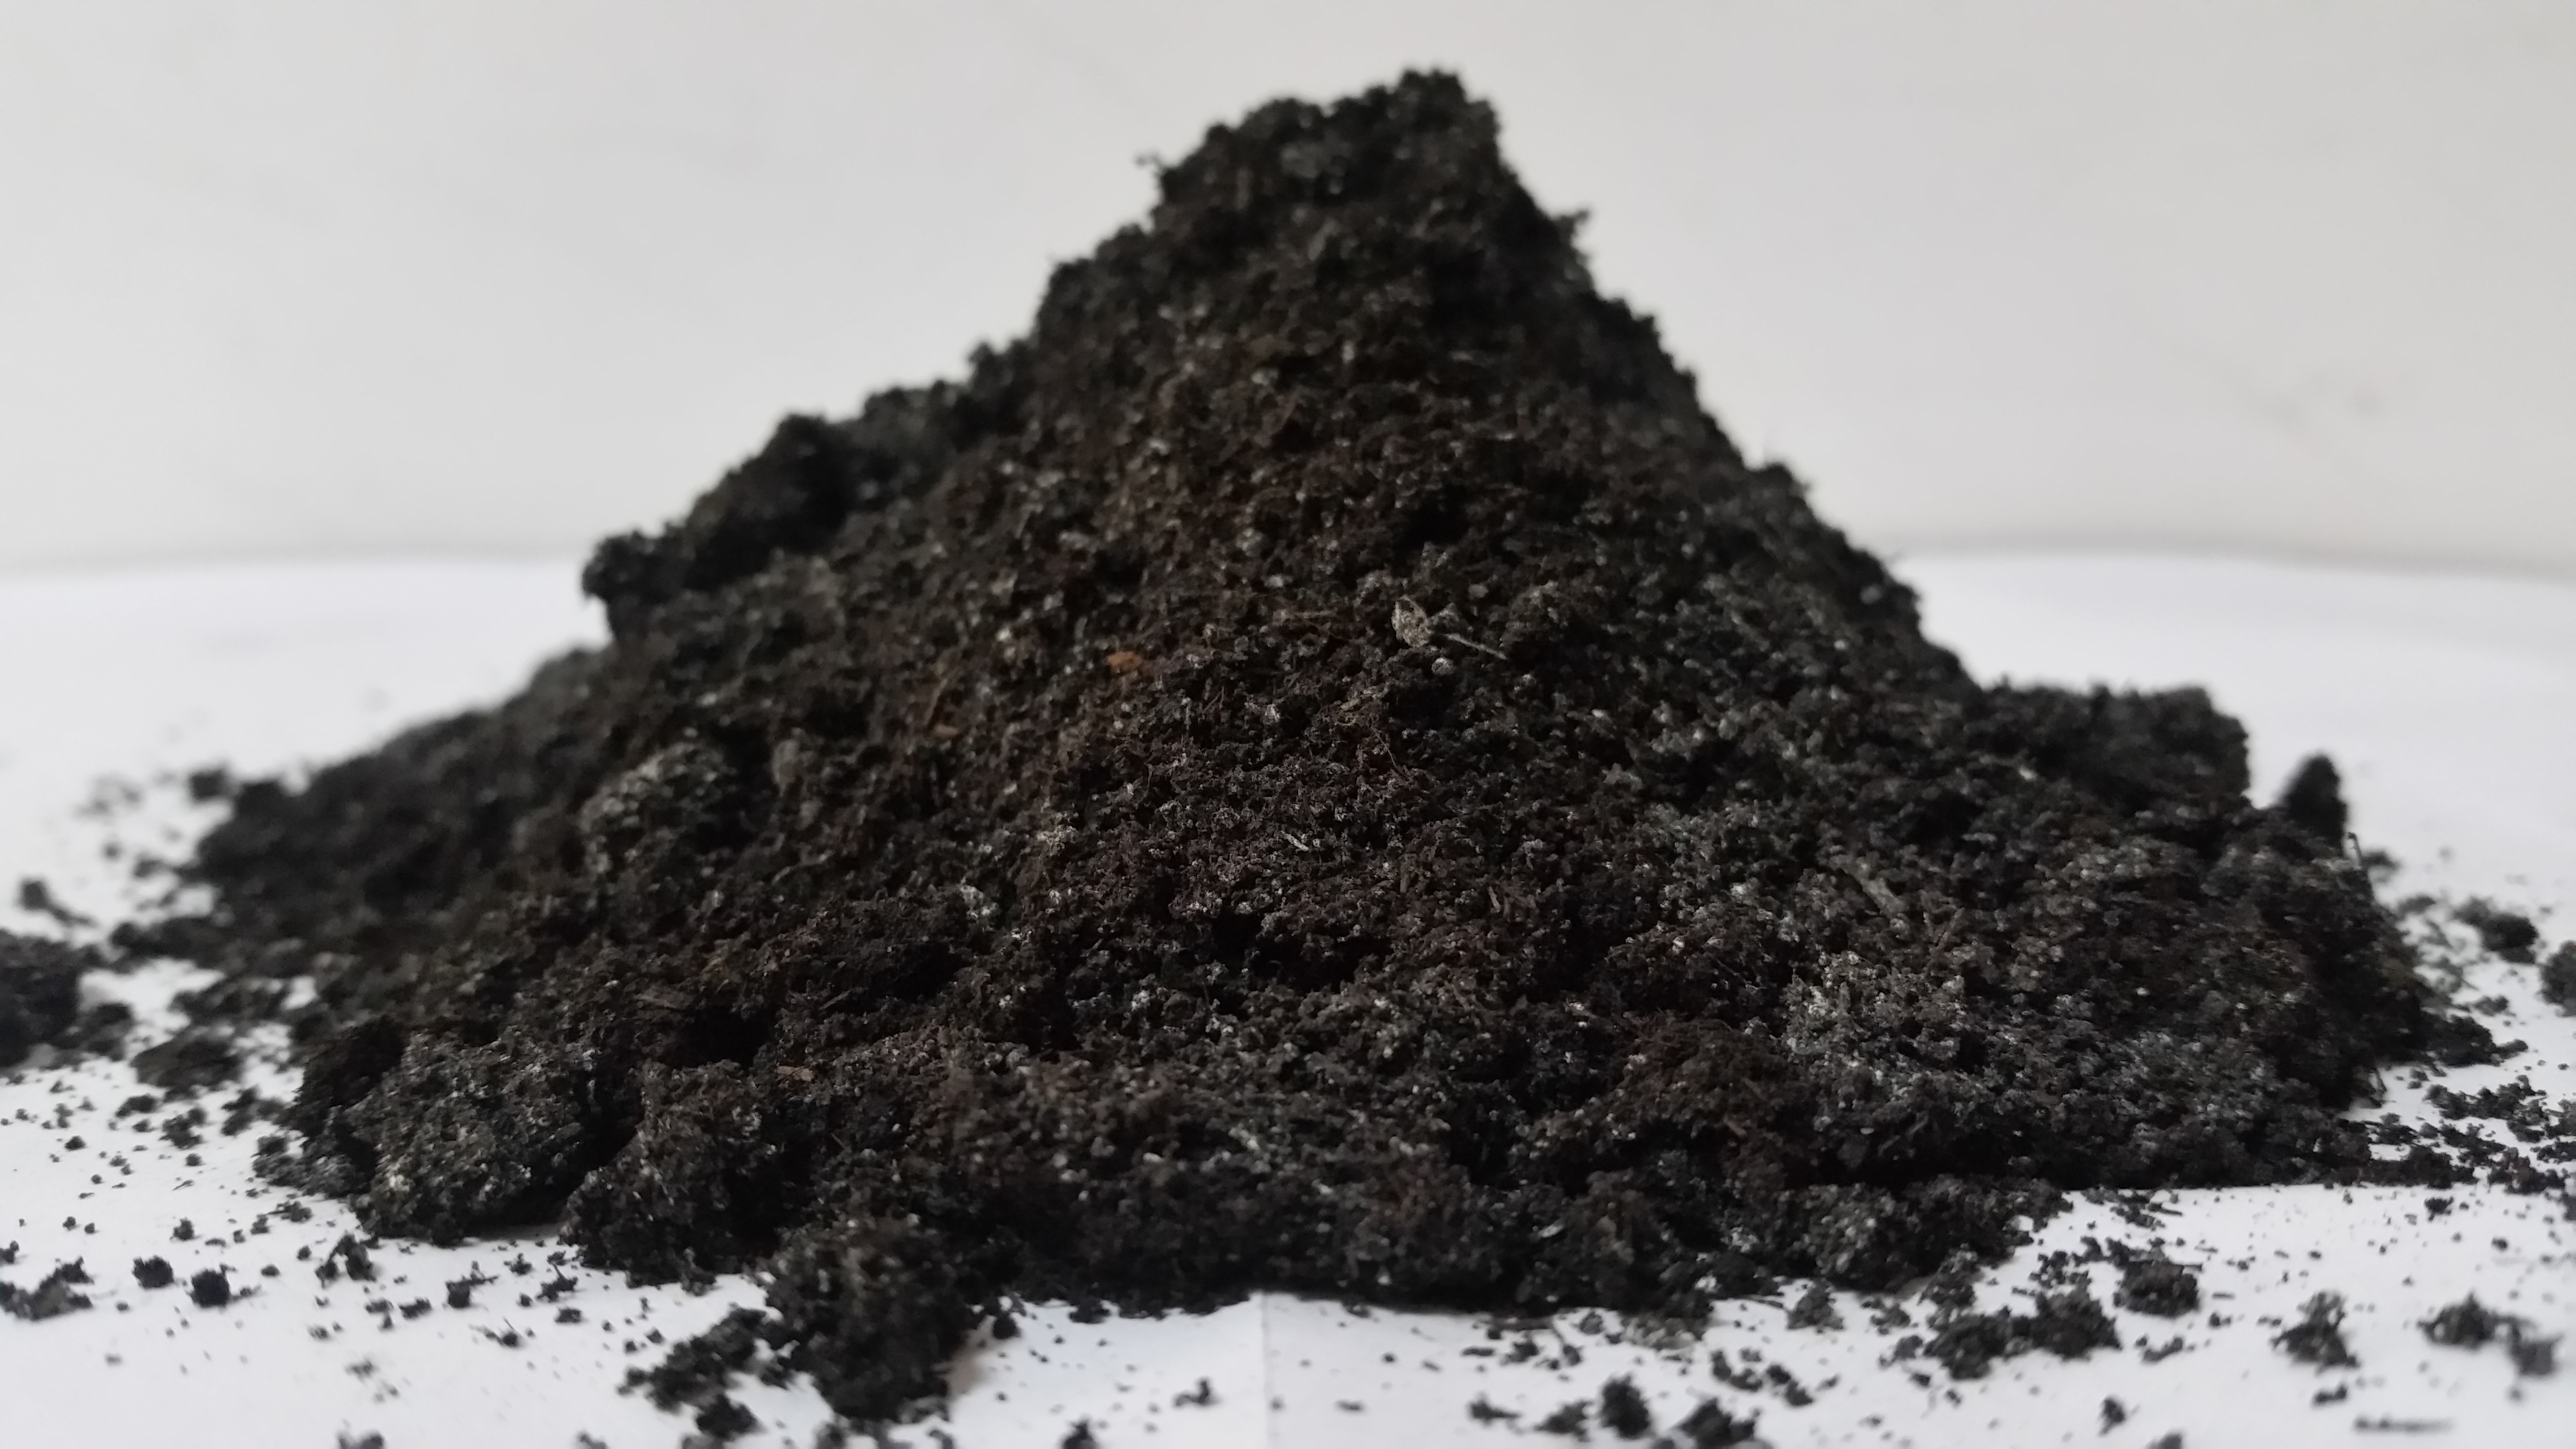
\includegraphics[width=0.4\textwidth]{../../assets/有机肥.png}
		\caption{有机肥}
		\label{pic:有机肥}
	\end{minipage}
\end{figure}

已有研究证明超声振动可在谐振频率范围内降低气缸的摩擦力，提高气缸控制精度\cite{__2023}。通过分析，我们可以将超声波振动应用到农业领域。